\documentclass[]{article}
\usepackage{amssymb,amsmath}
\usepackage{ifxetex,ifluatex}
\ifxetex
  \usepackage{fontspec,xltxtra,xunicode}
  \defaultfontfeatures{Mapping=tex-text,Scale=MatchLowercase}
\else
  \ifluatex
    \usepackage{fontspec}
    \defaultfontfeatures{Mapping=tex-text,Scale=MatchLowercase}
  \else
    \usepackage[utf8]{inputenc}
  \fi
\fi
\usepackage{ctable}
\usepackage{float} % provides the H option for float placement
\usepackage{graphicx}
% We will generate all images so they have a width \maxwidth. This means
% that they will get their normal width if they fit onto the page, but
% are scaled down if they would overflow the margins.
\makeatletter
\def\maxwidth{\ifdim\Gin@nat@width>\linewidth\linewidth
\else\Gin@nat@width\fi}
\makeatother
\let\Oldincludegraphics\includegraphics
\renewcommand{\includegraphics}[1]{\Oldincludegraphics[width=\maxwidth]{#1}}
\ifxetex
  \usepackage[setpagesize=false, % page size defined by xetex
              unicode=false, % unicode breaks when used with xetex
              xetex,
              colorlinks=true,
              linkcolor=blue]{hyperref}
\else
  \usepackage[unicode=true,
              colorlinks=true,
              linkcolor=blue]{hyperref}
\fi
\hypersetup{breaklinks=true, pdfborder={0 0 0}}
\setlength{\parindent}{0pt}
\setlength{\parskip}{6pt plus 2pt minus 1pt}
\setlength{\emergencystretch}{3em}  % prevent overfull lines
\setcounter{secnumdepth}{0}

\title{Correlations}
\author{Rapport package team @ https://github.com/aL3xa/rapport}
\date{2011-04-26 20:25 CET}

\begin{document}
\maketitle

\subsection{Description}

This template will return the correlation matrix of supplied numerical
variables.

\subsection{Variable description}

\emph{3} variables provided.

The highest correlation coefficient (0.2273) is between \emph{edu} and
\emph{age} and the lowest (-0.0338) is between \emph{leisure} and
\emph{age}. It seems that the strongest association (r=0.2273) is
between \emph{edu} and \emph{age}.

Higly correlated (r \textless{} 0.7 or r \textgreater{} 0.7) variables:
-

Uncorrelated (-0.2 \textless{} r \textless{} 0.2) variables:

\begin{itemize}
\item
  \emph{age} and \emph{leisure}
\item
  \emph{edu} and \emph{leisure}
\end{itemize}
\subsubsection{Correlation matrix}

\ctable[pos = H, center, botcap]{llll}
{% notes
}
{% rows
\FL
 & \textbf{age} & \textbf{edu} & \textbf{leisure}
\ML
age &  & 0.2273 * * * & -0.0338
\\\noalign{\medskip}
edu & 0.2273 * * * &  & 0.1732 * * *
\\\noalign{\medskip}
leisure & -0.0338 & 0.1732 * * * & 
\LL
}

\href{0e4cca7017b21223d68df3b9e300c895-hires.png}{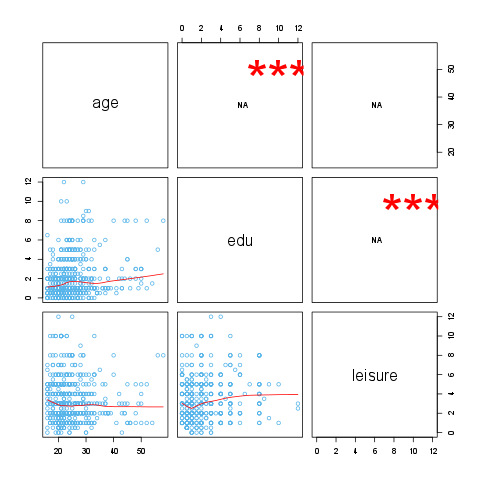
\includegraphics{0e4cca7017b21223d68df3b9e300c895.png}}

\subsection{Description}

This template will return the correlation matrix of supplied numerical
variables.

\subsection{Variable description}

\emph{11} variables provided.

The highest correlation coefficient (0.902) is between \emph{disp} and
\emph{cyl} and the lowest (-0.8677) is between \emph{wt} and \emph{mpg}.
It seems that the strongest association (r=0.902) is between \emph{disp}
and \emph{cyl}.

Higly correlated (r \textless{} 0.7 or r \textgreater{} 0.7) variables:

\begin{itemize}
\item
  \emph{mpg} and \emph{cyl}
\item
  \emph{mpg} and \emph{disp}
\item
  \emph{cyl} and \emph{disp}
\item
  \emph{mpg} and \emph{hp}
\item
  \emph{cyl} and \emph{hp}
\item
  \emph{disp} and \emph{hp}
\item
  \emph{disp} and \emph{drat}
\item
  \emph{mpg} and \emph{wt}
\item
  \emph{cyl} and \emph{wt}
\item
  \emph{disp} and \emph{wt}
\item
  \emph{drat} and \emph{wt}
\item
  \emph{hp} and \emph{qsec}
\item
  \emph{cyl} and \emph{vs}
\item
  \emph{disp} and \emph{vs}
\item
  \emph{hp} and \emph{vs}
\item
  \emph{qsec} and \emph{vs}
\item
  \emph{drat} and \emph{am}
\item
  \emph{am} and \emph{gear}
\item
  \emph{hp} and \emph{carb}
\end{itemize}
Uncorrelated (-0.2 \textless{} r \textless{} 0.2) variables:

\begin{itemize}
\item
  \emph{drat} and \emph{qsec}
\item
  \emph{wt} and \emph{qsec}
\item
  \emph{vs} and \emph{am}
\item
  \emph{hp} and \emph{gear}
\item
  \emph{drat} and \emph{carb}
\item
  \emph{am} and \emph{carb}
\end{itemize}
\subsubsection{Correlation matrix}

\ctable[pos = H, center, botcap]{llllllllllll}
{% notes
}
{% rows
\FL
 & \textbf{mpg} & \textbf{cyl} & \textbf{disp} & \textbf{hp} & \textbf{drat} & \textbf{wt} & \textbf{qsec} & \textbf{vs} & \textbf{am} & \textbf{gear} & \textbf{carb}
\ML
mpg &  & -0.8522 * * * & -0.8476 * * * & -0.7762 * * * & 0.6812 * *
* & -0.8677 * * * & 0.4187 * & 0.6640 * * * & 0.5998 * * * & 0.4803 *
* & -0.5509 * *
\\\noalign{\medskip}
cyl & -0.8522 * * * &  & 0.9020 * * * & 0.8324 * * * & -0.6999 * *
* & 0.7825 * * * & -0.5912 * * * & -0.8108 * * * & -0.5226 * * & -0.4927
* * & 0.5270 * *
\\\noalign{\medskip}
disp & -0.8476 * * * & 0.9020 * * * &  & 0.7909 * * * & -0.7102 * *
* & 0.8880 * * * & -0.4337 * & -0.7104 * * * & -0.5912 * * * & -0.5556 *
* * & 0.3950 *
\\\noalign{\medskip}
hp & -0.7762 * * * & 0.8324 * * * & 0.7909 * * * &  & -0.4488 *
* & 0.6587 * * * & -0.7082 * * * & -0.7231 * *
* & -0.2432 & -0.1257 & 0.7498 * * *
\\\noalign{\medskip}
drat & 0.6812 * * * & -0.6999 * * * & -0.7102 * * * & -0.4488 *
* &  & -0.7124 * * * & 0.0912 & 0.4403 * & 0.7127 * * * & 0.6996 * *
* & -0.0908
\\\noalign{\medskip}
wt & -0.8677 * * * & 0.7825 * * * & 0.8880 * * * & 0.6587 * *
* & -0.7124 * * * &  & -0.1747 & -0.5549 * * * & -0.6925 * * * & -0.5833
* * * & 0.4276 *
\\\noalign{\medskip}
qsec & 0.4187 * & -0.5912 * * * & -0.4337 * & -0.7082 * *
* & 0.0912 & -0.1747 &  & 0.7445 * * * & -0.2299 & -0.2127 & -0.6562 * *
*
\\\noalign{\medskip}
vs & 0.6640 * * * & -0.8108 * * * & -0.7104 * * * & -0.7231 * *
* & 0.4403 * & -0.5549 * * * & 0.7445 * *
* &  & 0.1683 & 0.2060 & -0.5696 * * *
\\\noalign{\medskip}
am & 0.5998 * * * & -0.5226 * * & -0.5912 * * * & -0.2432 & 0.7127 * *
* & -0.6925 * * * & -0.2299 & 0.1683 &  & 0.7941 * * * & 0.0575
\\\noalign{\medskip}
gear & 0.4803 * * & -0.4927 * * & -0.5556 * * * & -0.1257 & 0.6996 * *
* & -0.5833 * * * & -0.2127 & 0.2060 & 0.7941 * * * &  & 0.2741
\\\noalign{\medskip}
carb & -0.5509 * * & 0.5270 * * & 0.3950 * & 0.7498 * *
* & -0.0908 & 0.4276 * & -0.6562 * * * & -0.5696 * *
* & 0.0575 & 0.2741 & 
\LL
}

\href{82a0f381195bb4f50da3c943e264add1-hires.png}{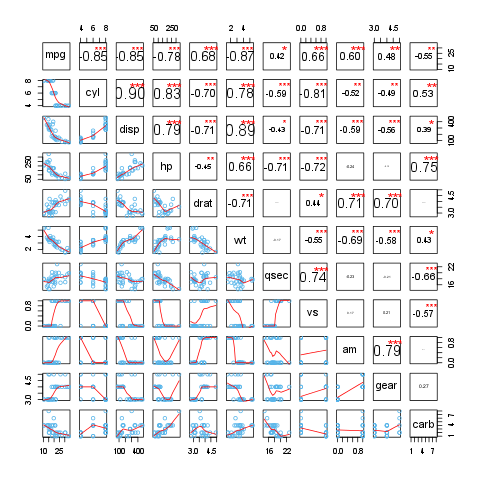
\includegraphics{82a0f381195bb4f50da3c943e264add1.png}}

\begin{center}\rule{3in}{0.4pt}\end{center}

This report was generated with \href{http://www.r-project.org/}{R}
(2.14.0) and \href{http://al3xa.github.com/rapport/}{rapport} (0.1) in
1.333 sec on x86\_64-unknown-linux-gnu platform.

\begin{figure}[htbp]
\centering

\includegraphics{images/logo.png}
\caption{}
\end{figure}

\end{document}
